\documentclass[11pt,a4paper]{report}
\usepackage{graphicx}
\usepackage[polish]{babel}
\usepackage[utf8]{inputenc}
\usepackage[T1]{fontenc}
\frenchspacing
\usepackage{indentfirst}
\usepackage{amsfonts}
\usepackage[nomarginpar, margin=.5in]{geometry}
\usepackage{subfig}

\author{Maciej Domagalski}
\title{Wyniki - warunek brzegowy}

\begin{document}

\chapter{Parametry}
\section{Dla obu algorytmów}
$$ t_0 = 7.5 \cdot 10^{-9}[s] $$
$$ \sigma_0 = 0.75 \cdot 10^{-9}[s] $$
$$ x \in [0, 2][m] $$
$$ L = 0.25 \cdot 10^{-6} \left[\frac{H}{m}\right] $$
$$ \mathbb{C} = 100 * 10^{-12}\left[\frac{F}{m}\right] $$
$$ R = 12.5[\Omega] $$
$$ G = 0.5 * 10^{-3}[s] $$
$$ R_{in} = 7.5[\Omega], R_{out} = 12.5[\Omega] $$
$$ c = \frac{1}{\sqrt{L \mathbb{C}}} \left[\frac{1}{s}\right] $$ 
$$ \Delta x = \frac{2 \cdot x_{max}}{10^4}[m] $$

\section{Dla algorytmu Monte Carlo}
$$ \sigma = 20 \cdot \Delta x $$
$$ \lambda = \frac{1}{2} \cdot \left( \frac{R}{L} - \frac{G}{\mathbb{C}} \right) $$ 
$$ \mu = \frac{G}{\mathbb{C}} $$
$$ R_0 = \sqrt{\frac{L}{C}} $$
$$ \gamma_{in} = \frac {Rin - R0} {Rin + R0}, \gamma_{out} = \frac {Rout - R0} {Rout + R0}  $$
$$ \xi = \frac {R0} {R0 + Rin} $$
\newpage

\chapter{Wykresy}

\begin{figure}
\begin{tabular}{ccc}
  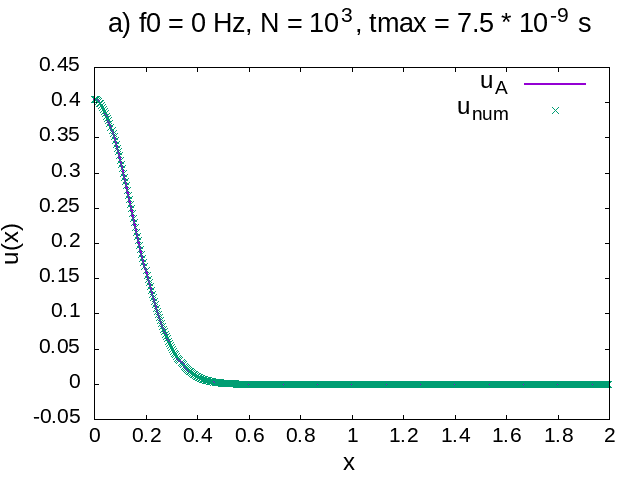
\includegraphics[width=55mm]{plots/0/mc0_3_075} &   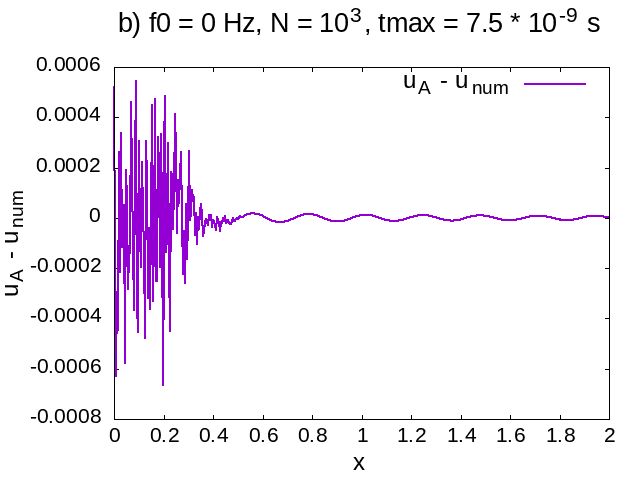
\includegraphics[width=55mm]{plots/0/mc0_3_075_dif} &   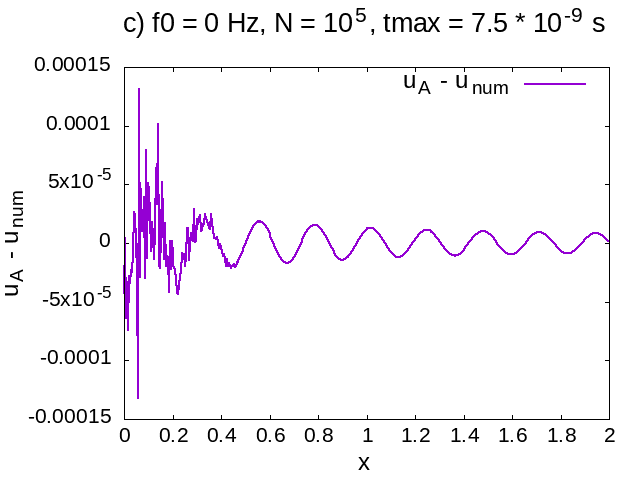
\includegraphics[width=55mm]{plots/0/mc0_5_075_dif} \\
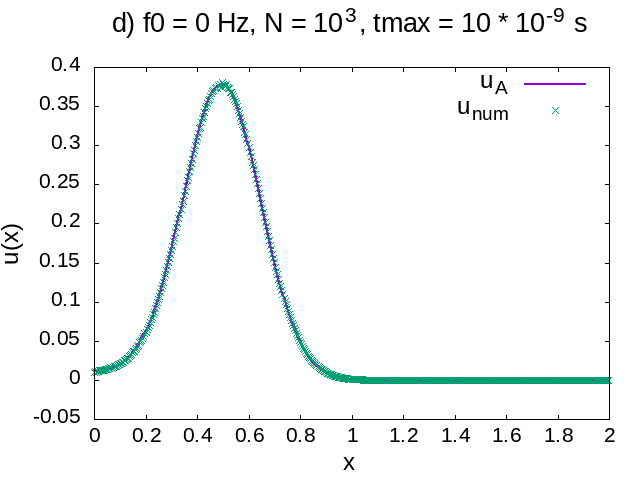
\includegraphics[width=55mm]{plots/0/mc0_3_10} &   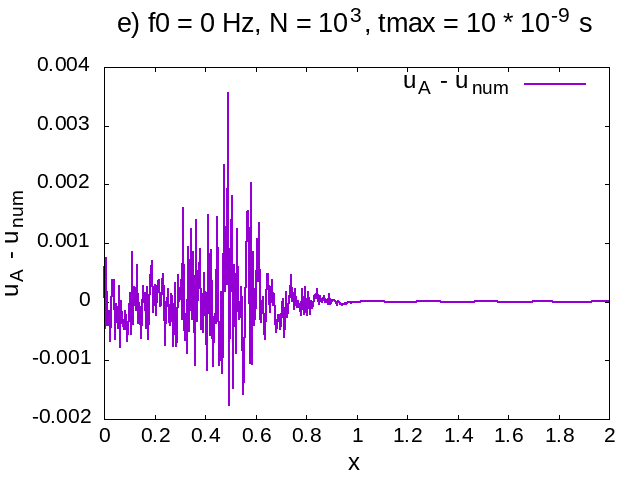
\includegraphics[width=55mm]{plots/0/mc0_3_10_dif} &   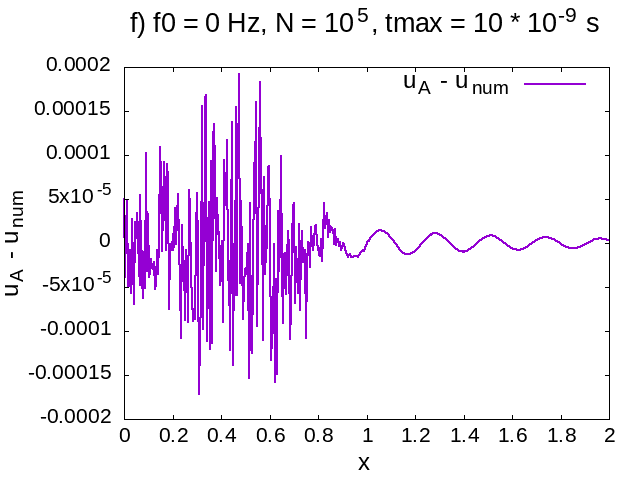
\includegraphics[width=55mm]{plots/0/mc0_5_10_dif} \\
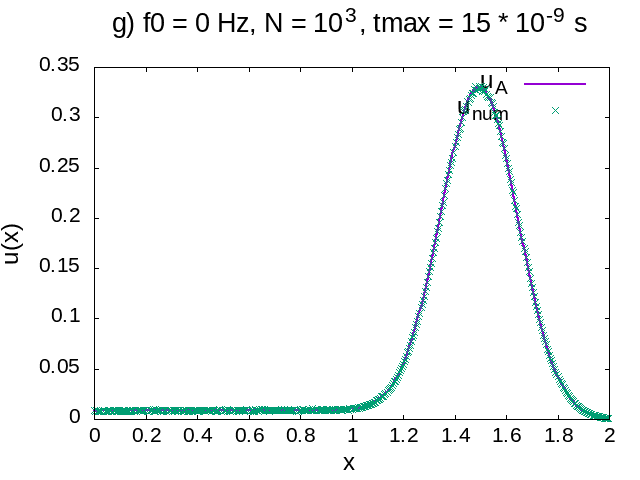
\includegraphics[width=55mm]{plots/0/mc0_3_15} &   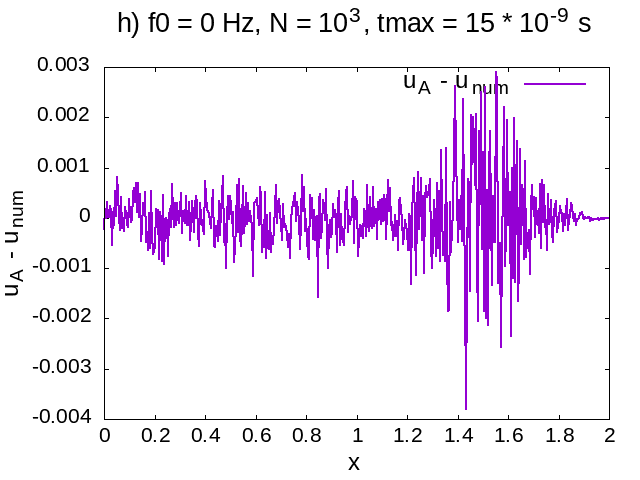
\includegraphics[width=55mm]{plots/0/mc0_3_15_dif} &   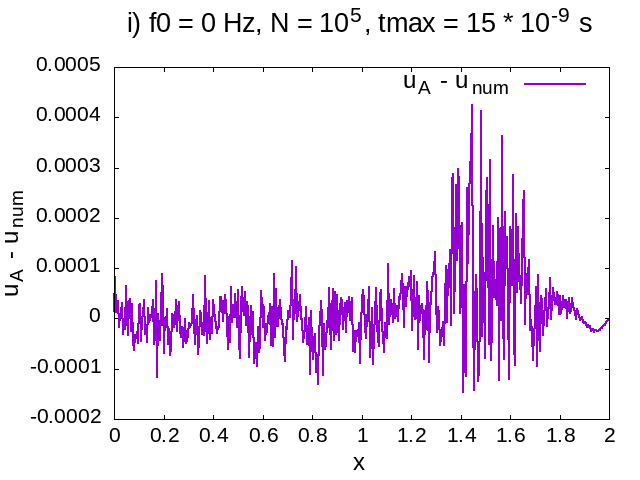
\includegraphics[width=55mm]{plots/0/mc0_5_15_dif} \\
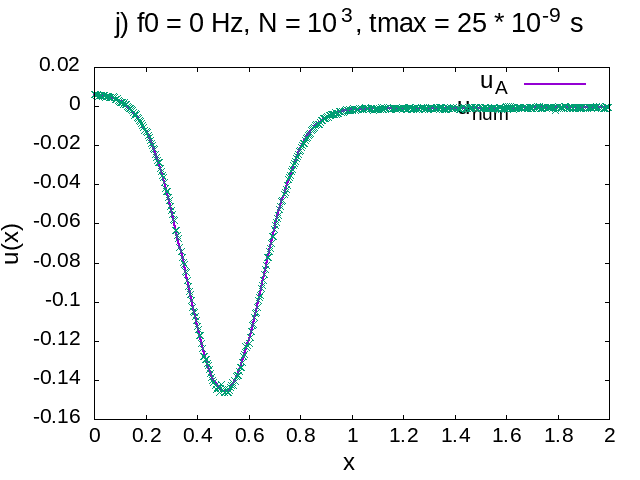
\includegraphics[width=55mm]{plots/0/mc0_3_25} &   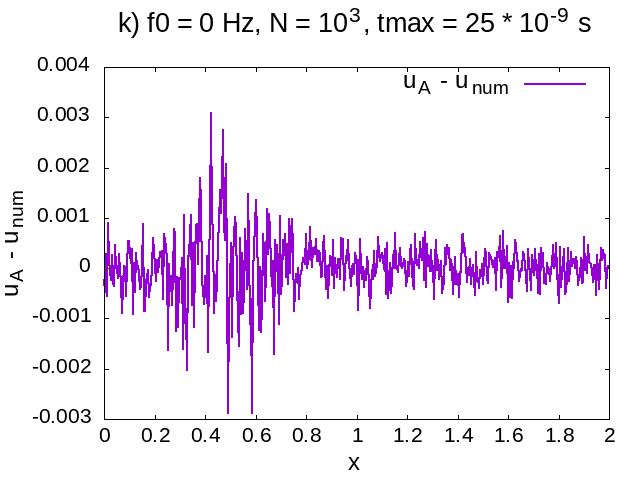
\includegraphics[width=55mm]{plots/0/mc0_3_25_dif} &   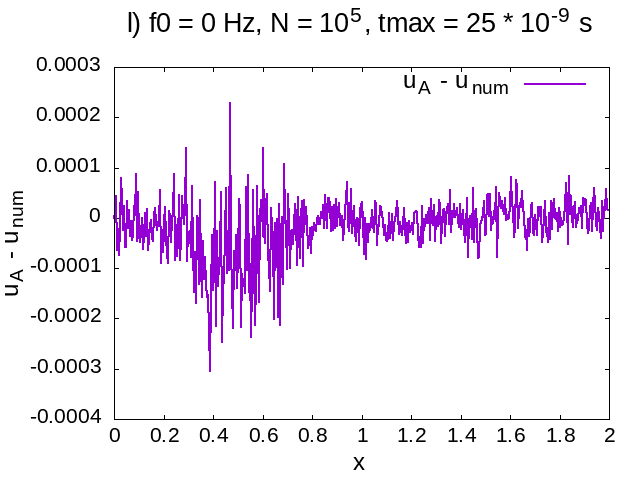
\includegraphics[width=55mm]{plots/0/mc0_5_25_dif} \\
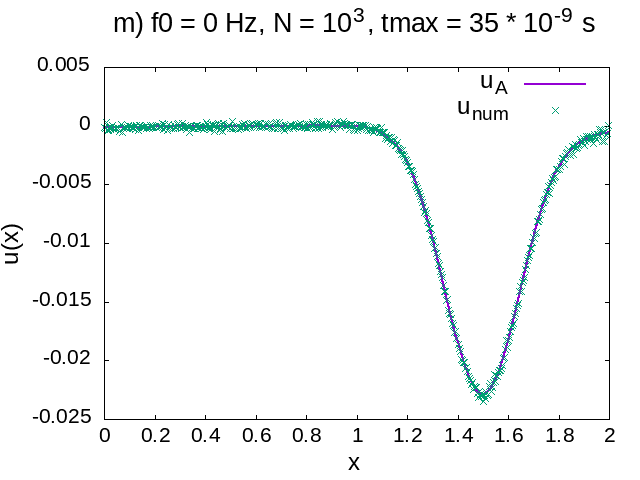
\includegraphics[width=55mm]{plots/0/mc0_3_35} &   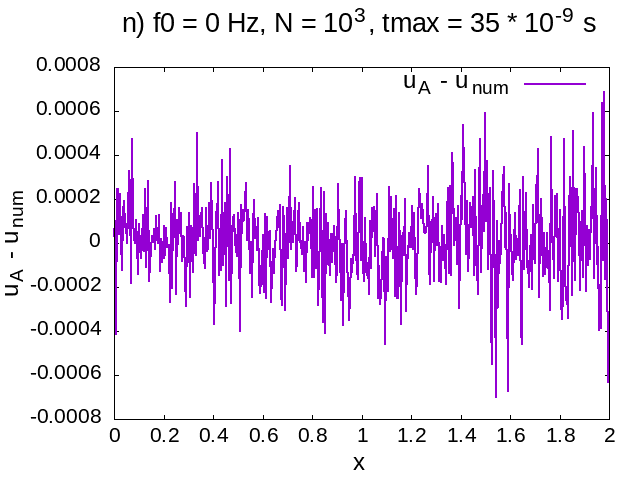
\includegraphics[width=55mm]{plots/0/mc0_3_35_dif} &   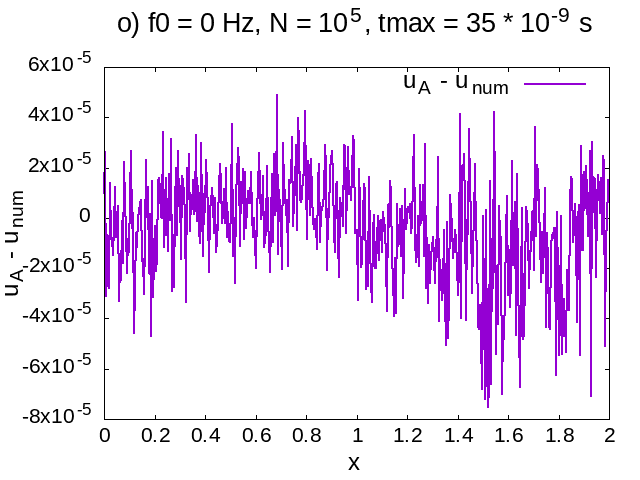
\includegraphics[width=55mm]{plots/0/mc0_5_35_dif} \\
\end{tabular}
\caption{Wyniki dla $f_0 = 0$. Wykres $u(x) = f(x)+b(x)$ dla $N = 10^3$, wykres błędu dla $10^3$ i $10^5$.}
\end{figure}
\newpage

\begin{figure}
\begin{tabular}{ccc}
  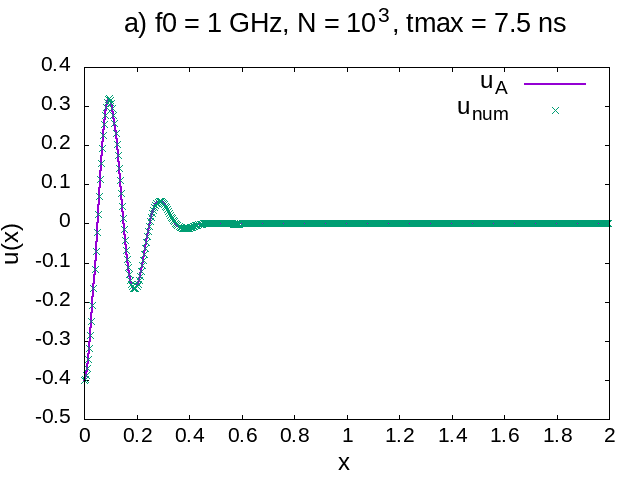
\includegraphics[width=55mm]{plots/1/mc1_3_075} &   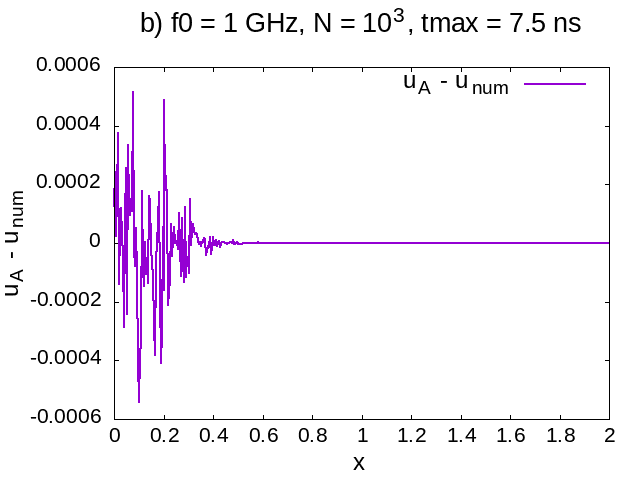
\includegraphics[width=55mm]{plots/1/mc1_3_075_dif} &   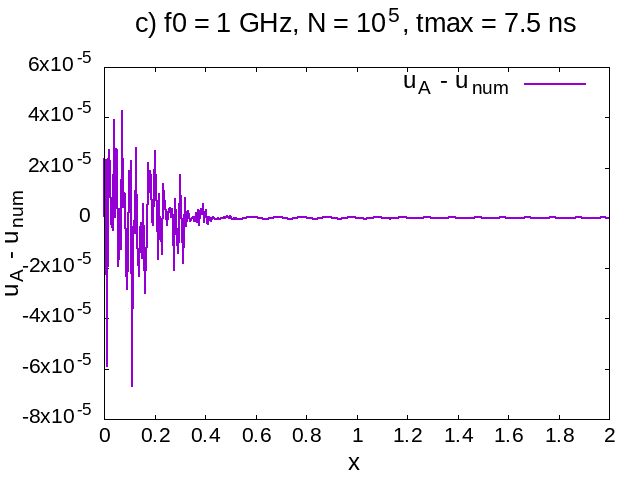
\includegraphics[width=55mm]{plots/1/mc1_5_075_dif} \\
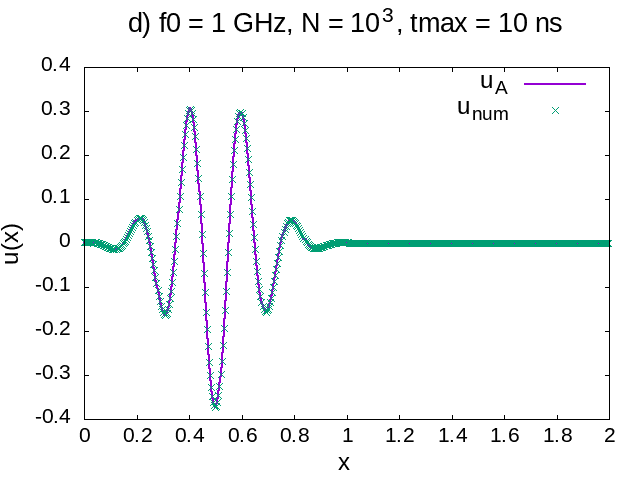
\includegraphics[width=55mm]{plots/1/mc1_3_10} &   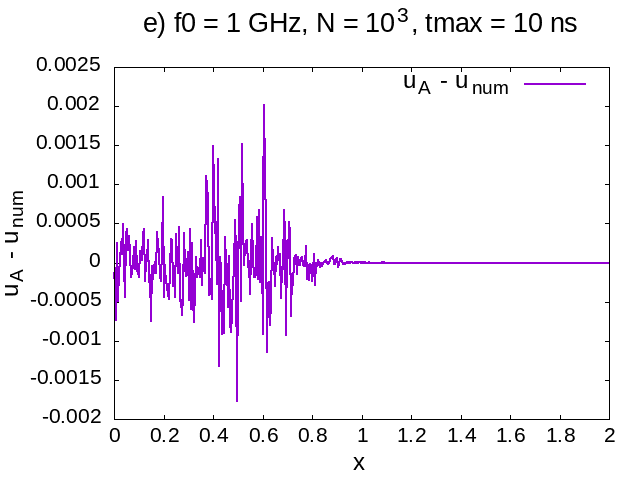
\includegraphics[width=55mm]{plots/1/mc1_3_10_dif} &   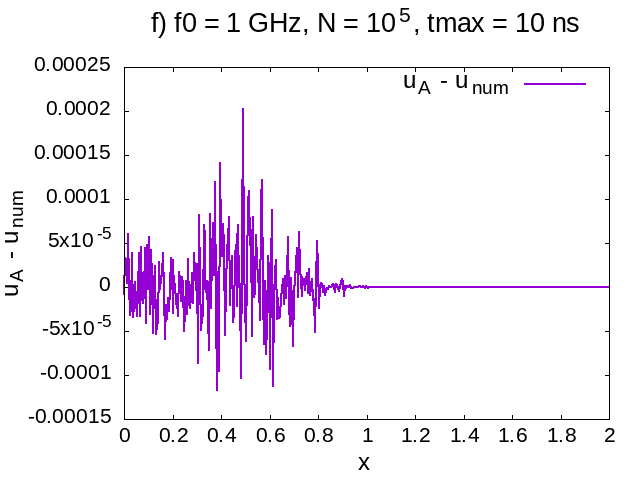
\includegraphics[width=55mm]{plots/1/mc1_5_10_dif} \\
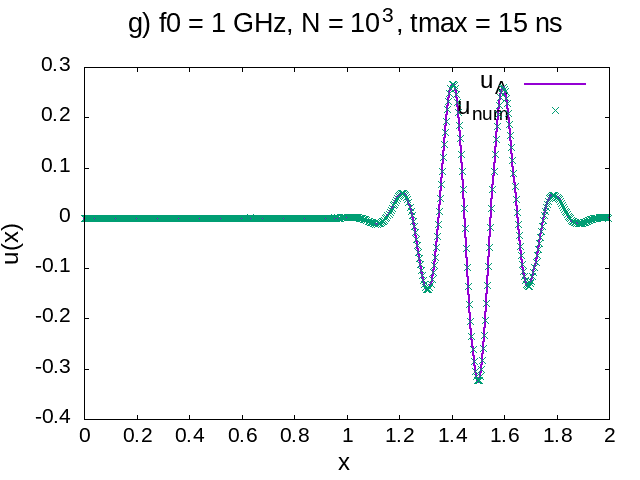
\includegraphics[width=55mm]{plots/1/mc1_3_15} &   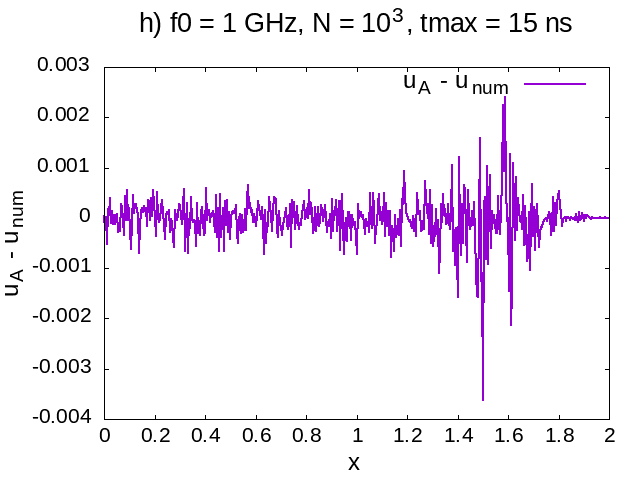
\includegraphics[width=55mm]{plots/1/mc1_3_15_dif} &   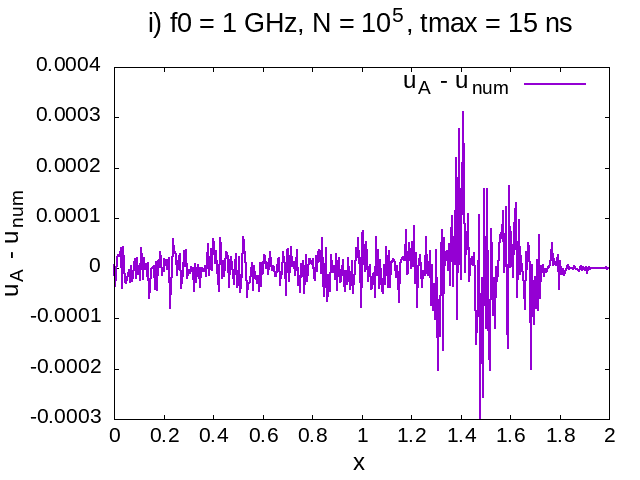
\includegraphics[width=55mm]{plots/1/mc1_5_15_dif} \\
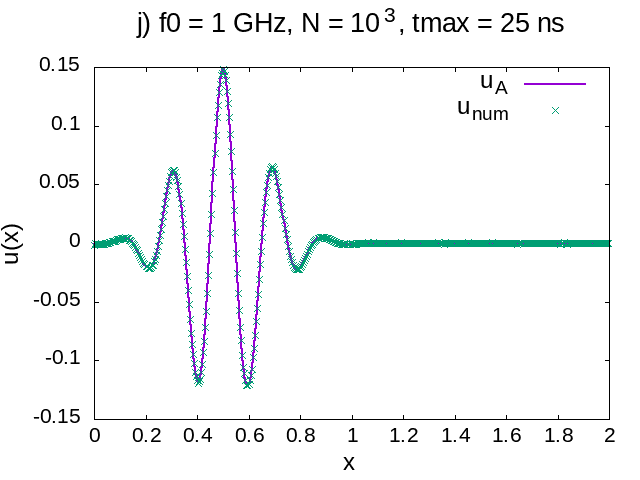
\includegraphics[width=55mm]{plots/1/mc1_3_25} &   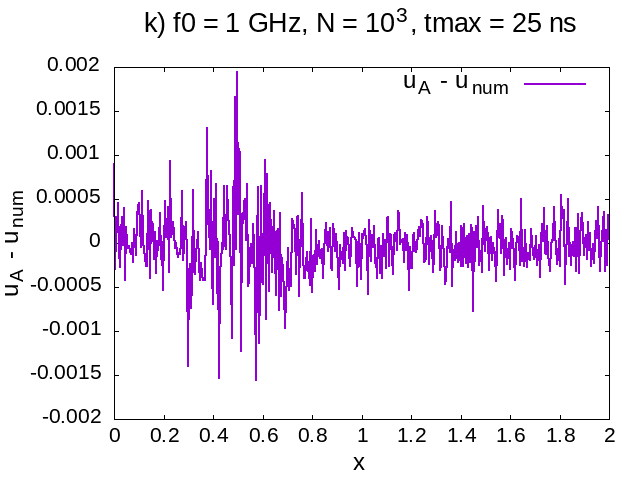
\includegraphics[width=55mm]{plots/1/mc1_3_25_dif} &   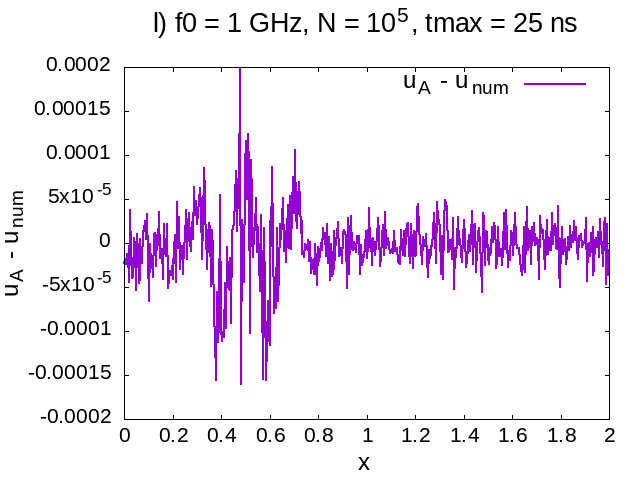
\includegraphics[width=55mm]{plots/1/mc1_5_25_dif} \\
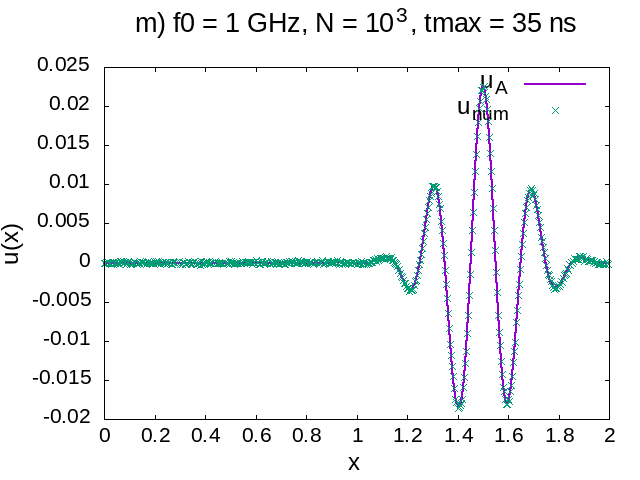
\includegraphics[width=55mm]{plots/1/mc1_3_35} &   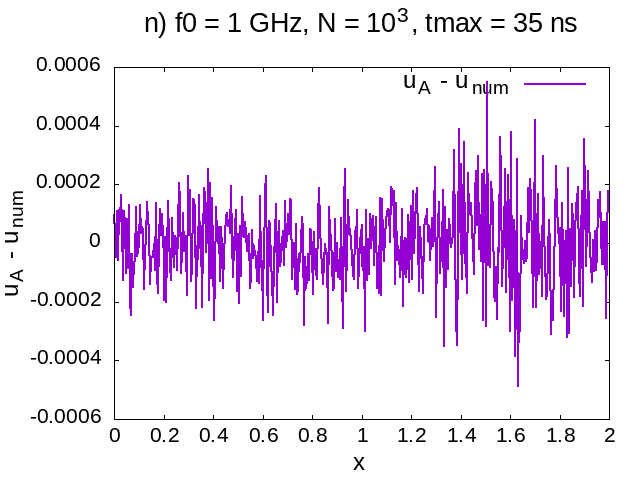
\includegraphics[width=55mm]{plots/1/mc1_3_35_dif} &   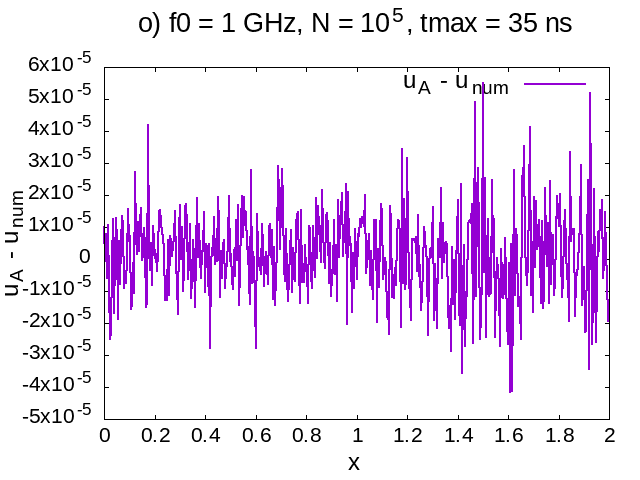
\includegraphics[width=55mm]{plots/1/mc1_5_35_dif} \\
\end{tabular}
\caption{Wyniki dla $f_0 = 1 \cdot 10^9$. Wykres $u(x) = f(x)+b(x)$ dla $N = 10^3$, wykres błędu dla $10^3$ i $10^5$.}
\end{figure}
\newpage

\begin{figure}
\begin{tabular}{ccc}
  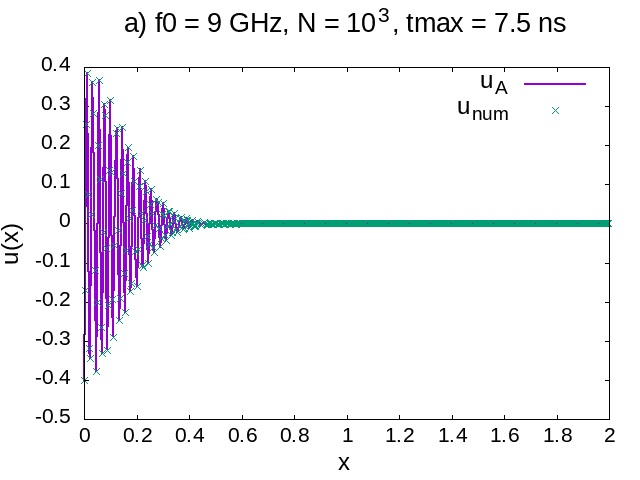
\includegraphics[width=55mm]{plots/9/mc9_3_075} &   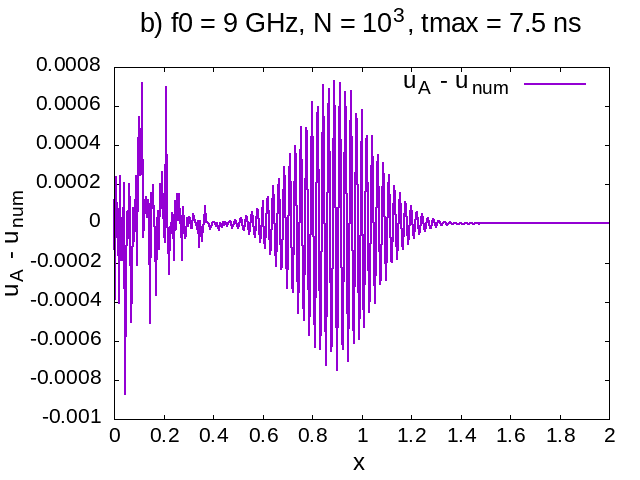
\includegraphics[width=55mm]{plots/9/mc9_3_075_dif} &   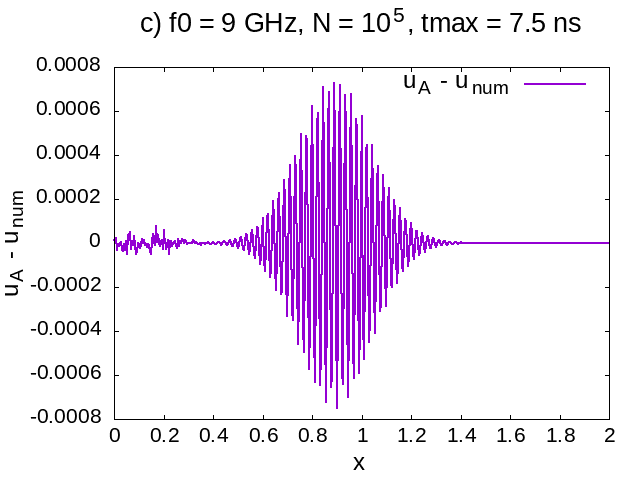
\includegraphics[width=55mm]{plots/9/mc9_5_075_dif} \\
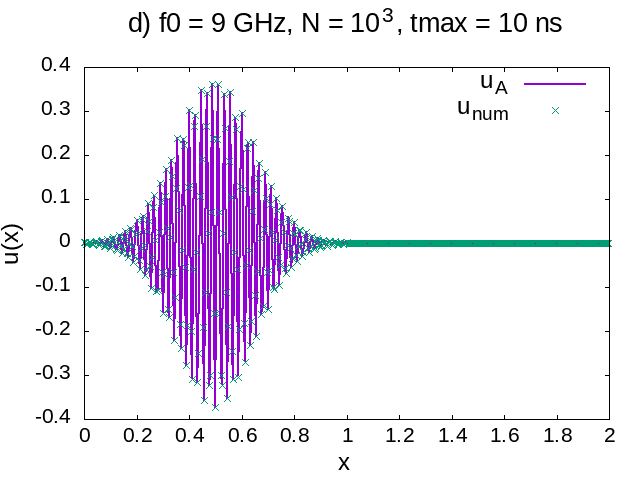
\includegraphics[width=55mm]{plots/9/mc9_3_10} &   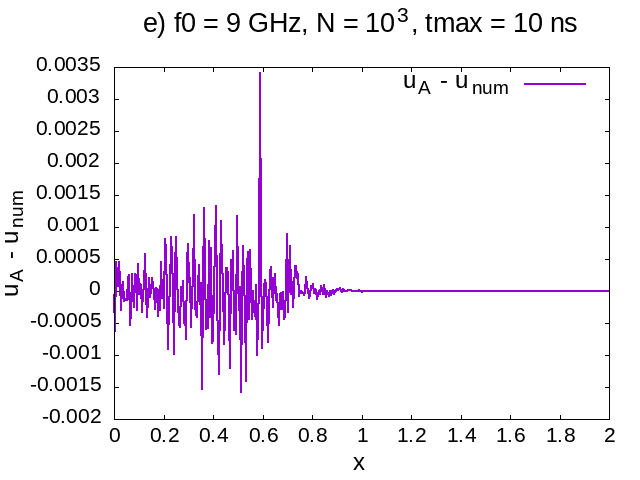
\includegraphics[width=55mm]{plots/9/mc9_3_10_dif} &   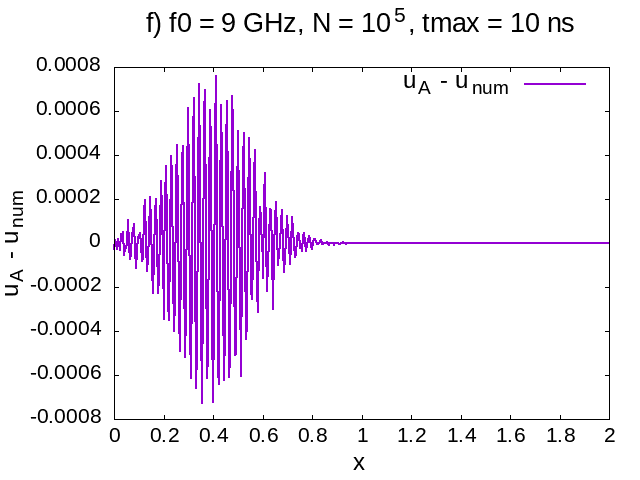
\includegraphics[width=55mm]{plots/9/mc9_5_10_dif} \\
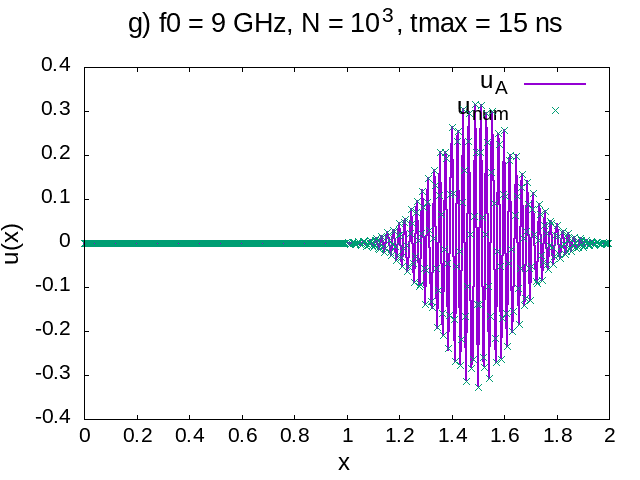
\includegraphics[width=55mm]{plots/9/mc9_3_15} &   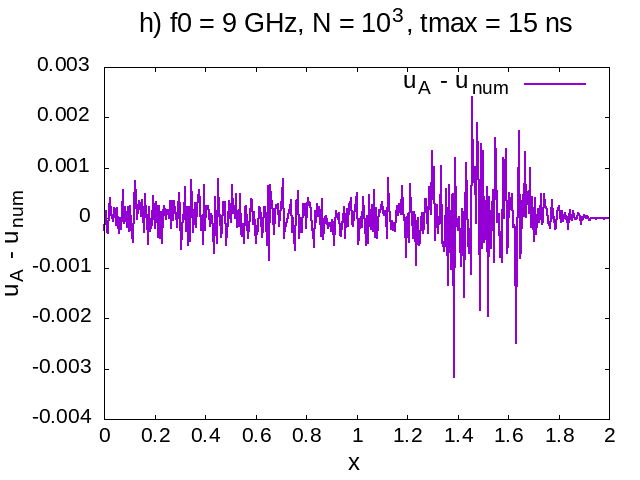
\includegraphics[width=55mm]{plots/9/mc9_3_15_dif} &   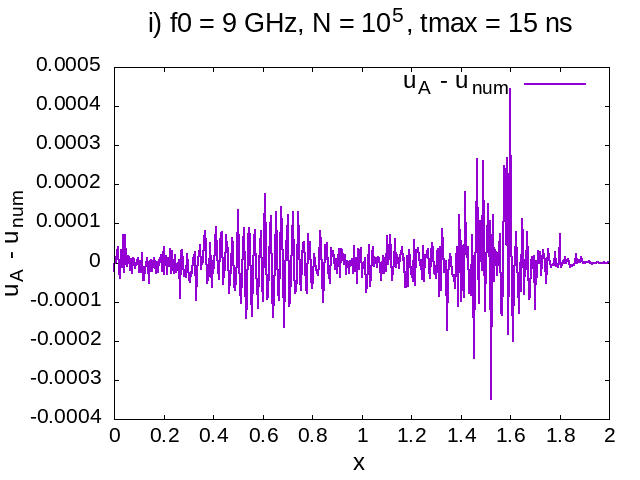
\includegraphics[width=55mm]{plots/9/mc9_5_15_dif} \\
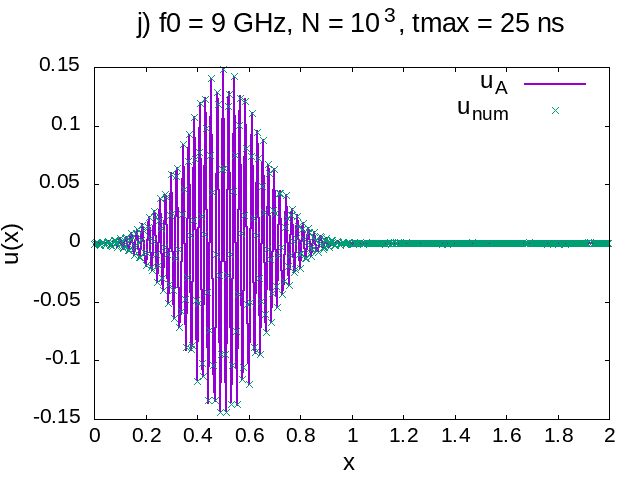
\includegraphics[width=55mm]{plots/9/mc9_3_25} &   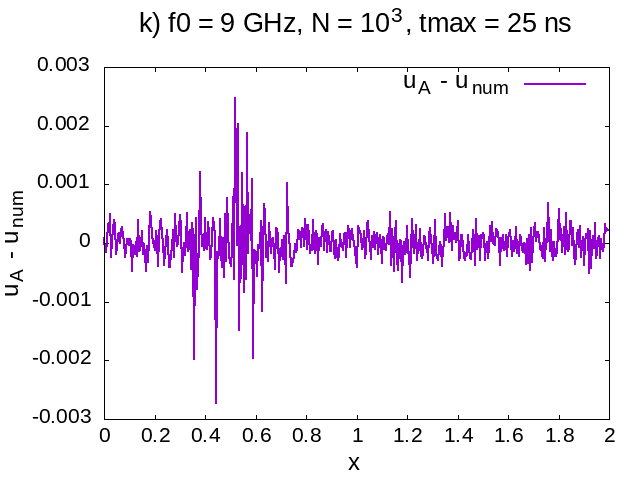
\includegraphics[width=55mm]{plots/9/mc9_3_25_dif} &   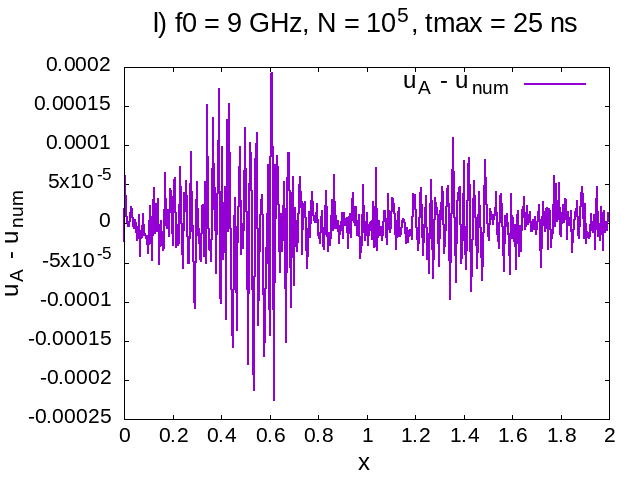
\includegraphics[width=55mm]{plots/9/mc9_5_25_dif} \\
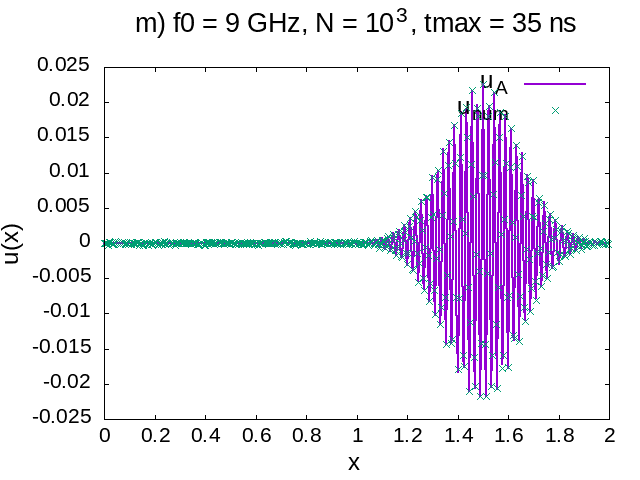
\includegraphics[width=55mm]{plots/9/mc9_3_35} &   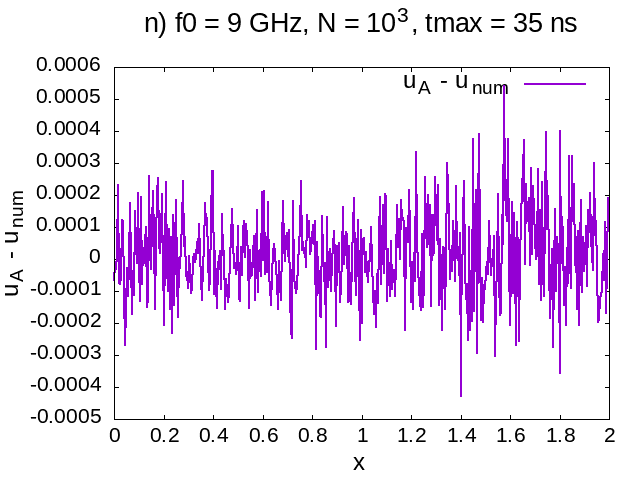
\includegraphics[width=55mm]{plots/9/mc9_3_35_dif} &   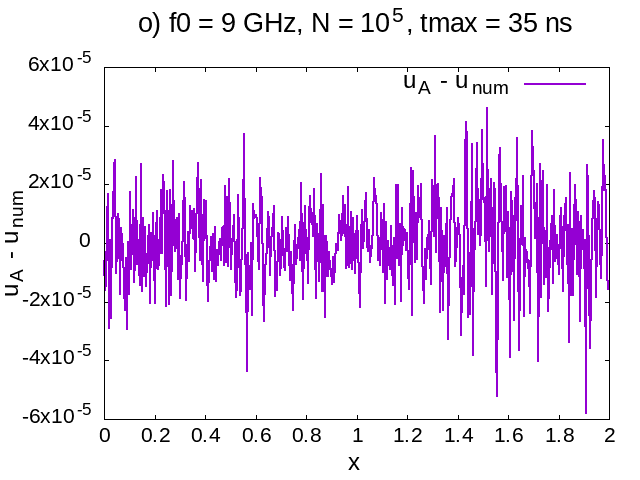
\includegraphics[width=55mm]{plots/9/mc9_5_35_dif} \\
\end{tabular}
\caption{Wyniki dla $f_0 = 9 \cdot 10^9$. Wykres $u(x) = f(x)+b(x)$ dla $N = 10^3$, wykres błędu dla $10^3$ i $10^5$.}
\end{figure}
\newpage

\begin{figure}
\begin{tabular}{cccc}
  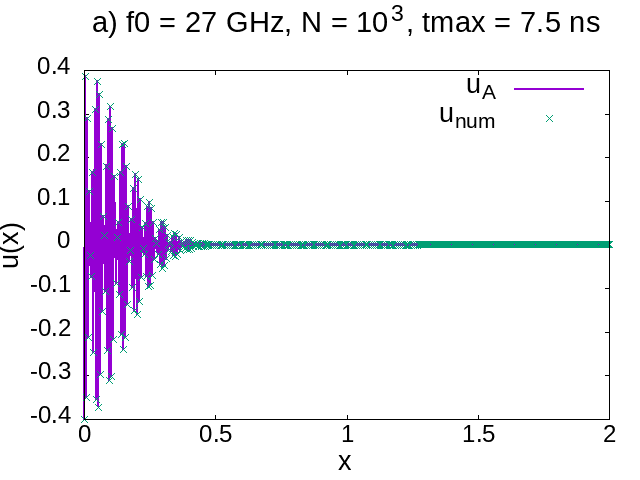
\includegraphics[width=45mm]{plots/27/mc27_3_075} & 
  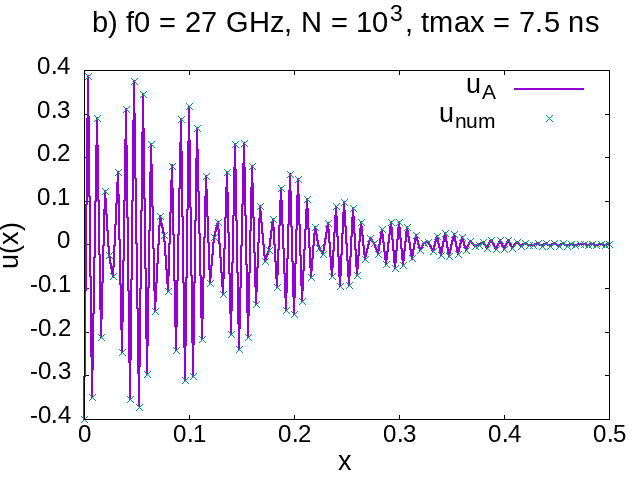
\includegraphics[width=45mm]{plots/27/closeup/mc27_3_075} &     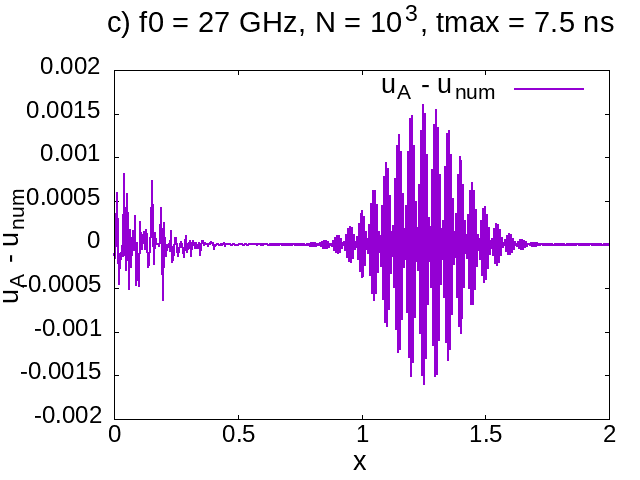
\includegraphics[width=45mm]{plots/27/mc27_3_075_dif} &   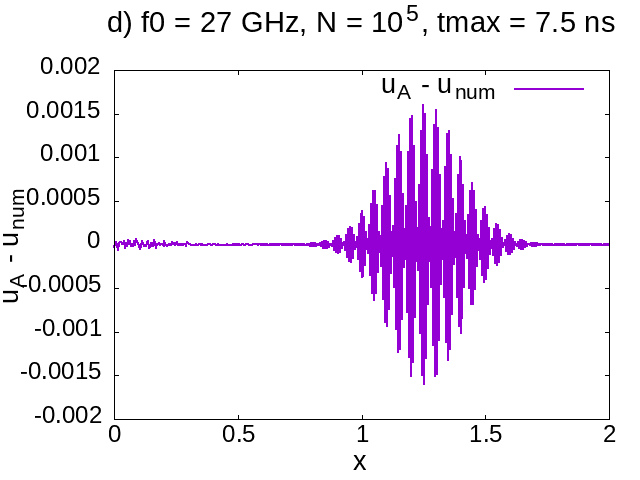
\includegraphics[width=45mm]{plots/27/mc27_5_075_dif} \\
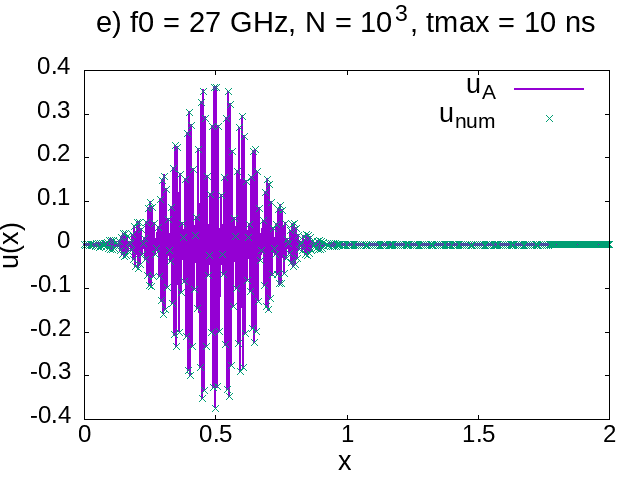
\includegraphics[width=45mm]{plots/27/mc27_3_10} &   
\includegraphics[width=45mm]{plots/27/closeup/mc27_3_10} &    \includegraphics[width=45mm]{plots/27/mc27_3_10_dif} &   \includegraphics[width=45mm]{plots/27/mc27_5_10_dif} \\
\includegraphics[width=45mm]{plots/27/mc27_3_15} &   
\includegraphics[width=45mm]{plots/27/closeup/mc27_3_15} &    \includegraphics[width=45mm]{plots/27/mc27_3_15_dif} &   \includegraphics[width=45mm]{plots/27/mc27_5_15_dif} \\
\includegraphics[width=45mm]{plots/27/mc27_3_25} & 
\includegraphics[width=45mm]{plots/27/closeup/mc27_3_25} &      \includegraphics[width=45mm]{plots/27/mc27_3_25_dif} &   \includegraphics[width=45mm]{plots/27/mc27_5_25_dif} \\
\includegraphics[width=45mm]{plots/27/mc27_3_35} &   
\includegraphics[width=45mm]{plots/27/closeup/mc27_3_35} &    \includegraphics[width=45mm]{plots/27/mc27_3_35_dif} &   \includegraphics[width=45mm]{plots/27/mc27_5_35_dif} \\
\end{tabular}
\caption{Wyniki dla $f_0 = 27 \cdot 10^9$. Wykres $u(x) = f(x)+b(x)$ dla $N = 10^3$ (w całym przedziale $x$ oraz w obszarze oscylacji). Wykres błędu dla $10^3$ i $10^5$.}
\end{figure}
\newpage

\chapter{Analiza jakościowa rozwiązań}

\begin{figure}
\begin{tabular}{cc}
  \includegraphics[width=75mm]{zad4/zad4_0} &   \includegraphics[width=75mm]{zad4/zad4_1} \\
  \includegraphics[width=75mm]{zad4/zad4_3} &   \includegraphics[width=75mm]{zad4/zad4_9} \\
  \includegraphics[width=75mm]{zad4/zad4_27} & \\
\end{tabular}
\caption{Największe odchylenia od wartości analitycznych dla danych wartości $N$ i $f_0$ w danej chwili $t$.}
\end{figure}
\newpage

\end{document}

\end{document}